\documentclass[20pt,mathserif]{beamer}

%Standarteinstellungen
\usepackage[english]{babel}
\usepackage[utf8x]{inputenc}
\usepackage[T1]{fontenc}

%Mathepackages
\usepackage{amsmath,amssymb,amsfonts,amsthm,mathtools}

%Tabellen tools
\usepackage{tabularx}
\usepackage{graphicx}

%Zeichnungen
\usepackage{tikz}
\usetikzlibrary{patterns,snakes}

%Anderthalbfacher Zeilenabstand
\usepackage{setspace}

%Farbe Section/Frametitles
\setbeamercolor{title}{fg=blue}
\setbeamercolor{frametitle}{fg=blue}

%Bulletpoints statt Bullettriangles
\setbeamertemplate{itemize item}[circle]

%Bulletpoints Farbe
\setbeamercolor{itemize item}{fg=blue} 

%Seitennummerierung
\setbeamertemplate{footline}[frame number] 

%Vordefinierte Umgebungen
\newtheorem{defi}{Definition}[subsection]
\newtheorem{satz}{Satz}[subsection]
\newtheorem{koro}{Korollar}[subsection]
\newtheorem{prop}{Proposition}[subsection] 

%Vordefinierte Befehle
\newcommand{\E}{\mathrm{E}}
\newcommand{\Var}{\mathrm{Var}}

%Erstllt Section Überschrift als Einzelnen Frame
\AtBeginSection[]{
	\begin{frame}
	\vfill
	\centering
	\begin{beamercolorbox}[sep=8pt,center,shadow=true,rounded=true]{title}
		\usebeamerfont{title}\insertsectionhead\par%
	\end{beamercolorbox}
	\vfill
\end{frame}
}

%Titelblatt
\title[Cross Validation]{ Linear Model selection by Cross-Validation}
%\subtitle{Researchmodule Econometrics}
\author{ Vivien Fritzsche, Jan Scherer, \\ Christoph Zilligen}
\date{\today}

\begin{document}
\beamertemplatenavigationsymbolsempty
\begin{frame}
\titlepage
\thispagestyle{empty}
\end{frame}

\begin{frame}
\frametitle{Motivating Example}
\centering
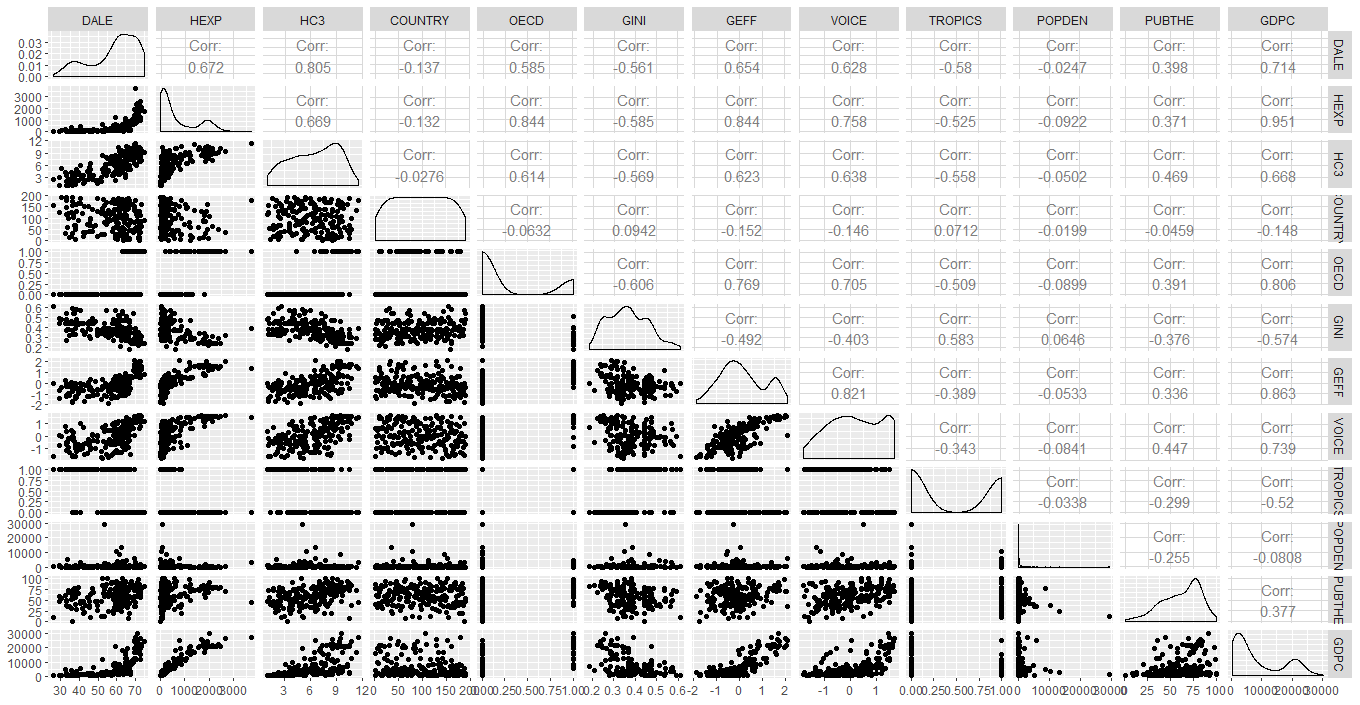
\includegraphics[width=1.25\textheight]{scatterplot.png}
\end{frame}
%Explain Example: Aim is ro estimate Liveexpectincy.Given some possible regressors.
%Scaterplott gets quickly comlicated for a growing number of regressors -> Therfore, we need a numeric procedure in order to select the model with best prediction ability.
%%Christoph%%

\thispagestyle{empty}
\section{General Framework and Notation}

\begin{frame}
\frametitle{Linear Setting}
\[
	y_i=x_i^\prime\beta+\varepsilon_i
\]
$x_i\in \mathbb{R}^p$ deterministic, $\varepsilon_i$ iid \\\vspace*{5pt}
$\E[\varepsilon_i]=0$\\\vspace*{5pt}
$\Var(\varepsilon_i)=\sigma^2<\infty$
\end{frame}
%We always consider a linear framework:,...,
%Some of the Betas might be zero and wie want to find out which of them are
%For simplicity we assume x_i to be deterministic, note that the whole argumentation would also work with probabilistic x_i
%%Vivien%%

\begin{frame}
\frametitle{Notation}
$\mathcal{M}_\alpha$ submodel:
\[
	y_i=x_{i,\alpha}^\prime\beta_\alpha+\varepsilon_i
\]
with $\alpha\subseteq\{1,\ldots,p\}$\\\vspace*{5pt}
and $\mathcal{M}_\ast$ as true model\\\vspace*{5pt}
$\hat{\beta}_\alpha$ is the OLS estimator
\end{frame}
%Introduce our notation of submodels
%There are 2^p-1 diffrent variations of diffrent models out of p regressors.
%To explain the structer of the submodels, Example Blackboard
%M_\ast denotes the true model.
%%Vivien%%

\thispagestyle{empty}
\section{Methods for Model Selection}

\begin{frame}
\frametitle{Popular Methods}

\begin{align*}
&\Gamma_\alpha=\E\left[||y-\hat{y}_\alpha||^2\right]
\\\\
&AIC_\alpha = 2k - 2\ln(\hat{L}_\alpha)\hspace{30cm}
\\\\
&BIC_\alpha = \ln(n)k - 2\ln(\hat{L}_\alpha)
\end{align*}
\end{frame}
%Beside Cross Validation, there are several other way's in order to do model selection. Mention: t-test, F-test,R squared,.... But the most popular (or most often used) are Bic and Aic.
%Due to theire basic aproach BIC, AIC and CV are very similar. 
%All three methods/criterion estimate the Expected squared prediction error for the different model variations. The model with the smallest Prediction error is chosen.
%AIC and BIC use alle date points for both, validation and construction inorder to estimate the Prediction error.(Last term of the equation). Since this leeds to a bias (overfitting) we need a correction term (first term)
%AIC and BIC only differ in this correction term 
%%Vivien$$

\begin{frame}
\frametitle{Cross Validation}
\vspace*{1.5cm}
\begin{overprint}
	\only<+>{
	
\begin{tikzpicture}
		\node at (0,0)[draw,inner sep=0.8em, fill = gray]{} ;
		\node at (2,0)[draw,inner sep=0.8em, fill = gray]{} ;
		\node at (4,0)[draw,inner sep=0.8em, fill = gray]{} ;
		\node at (6,0)[draw,inner sep=0.8em, fill = gray]{} ;
		\node at (8,0)[draw,inner sep=0.8em,fill = red,label= below:{\tiny validation}]{} ;
		\node at (10,0)[draw,inner sep=0.8em,fill =red,label= below:{\tiny validation}]{} ;
	\end{tikzpicture}
	\vspace*{70cm}
	}
	\only<+>{
		
\begin{tikzpicture}
		\node at (0,0)[draw,inner sep=0.8em, fill = gray]{} ;
		\node at (2,0)[draw,inner sep=0.8em, fill = gray]{} ;
		\node at (4,0)[draw,inner sep=0.8em, fill = gray]{} ;
		\node at (6,0)[draw,inner sep=0.8em,fill = red, label= below:{\tiny validation}]{} ;
		\node at (8,0)[draw,inner sep=0.8em, fill =gray]{} ;
		\node at (10,0)[draw,inner sep=0.8em,fill =red,label= below:{\tiny validation}]{} ;
		\end{tikzpicture}
		\vspace*{70cm}
	}
	\only<+>{
		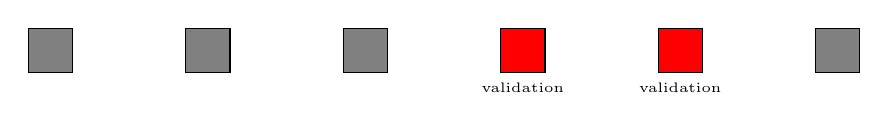
\begin{tikzpicture}
		\node at (0,0)[draw,inner sep=0.8em, fill = gray]{} ;
		\node at (2,0)[draw,inner sep=0.8em, fill = gray]{} ;
		\node at (4,0)[draw,inner sep=0.8em, fill = gray]{} ;
		\node at (6,0)[draw,inner sep=0.8em,fill = red, label= below:{\tiny validation}]{} ;
		\node at (8,0)[draw,inner sep=0.8em,fill =red,label= below:{\tiny validation}]{} ;
		\node at (10,0)[draw,inner sep=0.8em, fill = gray]{} ;
		\end{tikzpicture}
		\vspace*{70cm}
	}
	\only<+>{
		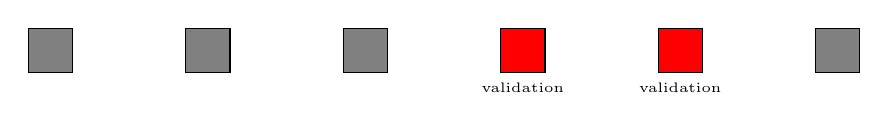
\begin{tikzpicture}
		\node at (0,0)[draw,inner sep=0.8em, fill = gray]{} ;
		\node at (2,0)[draw,inner sep=0.8em, fill = gray]{} ;
		\node at (4,0)[draw,inner sep=0.8em, fill = gray]{} ;
		\node at (6,0)[draw,inner sep=0.8em,fill = red, label= below:{\tiny validation}]{} ;
		\node at (8,0)[draw,inner sep=0.8em,fill =red,label= below:{\tiny validation}]{} ;
		\node at (10,0)[draw,inner sep=0.8em, fill = gray]{} ;
		\end{tikzpicture}
		\begin{align*}
		&CV_\alpha={\color{white} |P|^{-1}\sum_{s \in P}}\underbrace{n^{-1}_\nu||y_s-\hat{y}_{\alpha,s^c} ||^2}_{\hat{\Gamma}_{\alpha,s}} &\hspace{15cm}&
		\end{align*}
		\vspace{20cm}
	}
	\only<+>{
		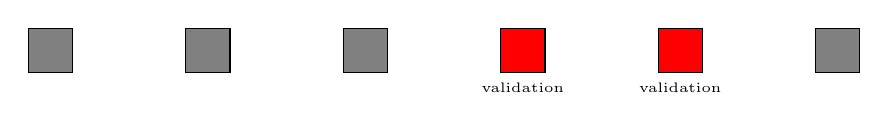
\begin{tikzpicture}
		\node at (0,0)[draw,inner sep=0.8em, fill = gray]{} ;
		\node at (2,0)[draw,inner sep=0.8em, fill = gray]{} ;
		\node at (4,0)[draw,inner sep=0.8em, fill = gray]{} ;
		\node at (6,0)[draw,inner sep=0.8em,fill = red, label= below:{\tiny validation}]{} ;
		\node at (8,0)[draw,inner sep=0.8em,fill =red,label= below:{\tiny validation}]{} ;
		\node at (10,0)[draw,inner sep=0.8em, fill = gray]{} ;
		\end{tikzpicture}
		\begin{align*}
		&CV_\alpha={\color{red} |P|^{-1}\sum_{s \in P}}\underbrace{n^{-1}_\nu||y_s-\hat{y}_{\alpha,s^c} ||^2}_{\hat{\Gamma}_{\alpha,s}} &\hspace{15cm}&
		\end{align*}
		\vspace{20cm}
	}
	\only<+>{
		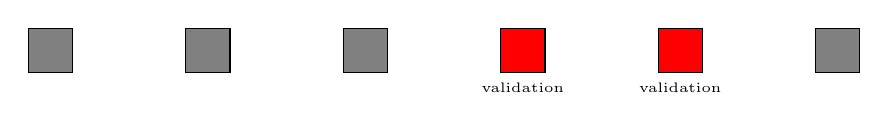
\begin{tikzpicture}
		\node at (0,0)[draw,inner sep=0.8em, fill = gray]{} ;
		\node at (2,0)[draw,inner sep=0.8em, fill = gray]{} ;
		\node at (4,0)[draw,inner sep=0.8em, fill = gray]{} ;
		\node at (6,0)[draw,inner sep=0.8em,fill = red, label= below:{\tiny validation}]{} ;
		\node at (8,0)[draw,inner sep=0.8em,fill =red,label= below:{\tiny validation}]{} ;
		\node at (10,0)[draw,inner sep=0.8em, fill = gray]{} ;
		\end{tikzpicture}
		\begin{align*}
		&CV_\alpha=\color{red}\underbrace{{\color{red} |P|^{-1}\sum_{s \in P}}{\color{black}\underbrace{n^{-1}_\nu||y_s-\hat{y}_{\alpha,s^c} ||^2}_{\hat{\Gamma}_{\alpha,s}}} }_{\hat{\Gamma}_\alpha}&\hspace{15cm}&
		\end{align*}
		\vspace{20cm}
	}
		\only<+>{
		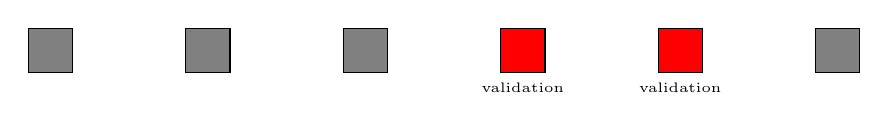
\begin{tikzpicture}
		\node at (0,0)[draw,inner sep=0.8em, fill = gray]{} ;
		\node at (2,0)[draw,inner sep=0.8em, fill = gray]{} ;
		\node at (4,0)[draw,inner sep=0.8em, fill = gray]{} ;
		\node at (6,0)[draw,inner sep=0.8em,fill = red, label= below:{\tiny validation}]{} ;
		\node at (8,0)[draw,inner sep=0.8em,fill =red,label= below:{\tiny validation}]{} ;
		\node at (10,0)[draw,inner sep=0.8em, fill = gray]{} ;
		\end{tikzpicture}
		\begin{align*}
		&CV_\alpha=|P|^{-1}\sum_{s\in P}n_\nu^{-1}||y_s-\hat{y}_{\alpha,s^c}||^2&\hspace{15cm}&
		\end{align*}
		\vspace{20cm}
	}
\end{overprint}
\end{frame}
%The main different of CV in comarisen to AIC and BIC is the way of sample spliting,
%CV devides the observations into a construction/trainingsample and a validation sample (see Example)
%Construction Sample -> To calculat the OLS Estimator... Validation -> Assesing the Prediction ability's/performance....
%For example for N=6 we can split into n_s=4 and n_v=2
%Claim that their (n over n_v) different ways of splitting the data,i.e, (n_v over n) different Partitions

%As already claimed CV estimates the expected squared pred error by simple empirical average.
%To reduce variance we calculate this estimate for every possible portion and calculate the average again
%CV does this for every \alpha and chooses the \alpha with the smallest error
%%Vivien%%

\begin{frame}
\frametitle{CV Variants}
\setlength{\tabcolsep}{1pt}
\begin{tabular}{ll}
	CV:& $P=\{s\subset\{1,\ldots,n\}|\#s= n_\nu\}$\\\\
	BICV:& $\mathcal{B}\subset P $ s.t $\# \mathcal{B}=b$\\\\
	MCCV:& $\mathcal{B}\subset P$ s.t $\# \mathcal{B}=b$
\end{tabular}
\end{frame}
%Their are different variations of CV.
%They only differ in the way of sample splitting
%Leave n_v out considers all possible spitings for a given n_v. Pro:it uses all possible information. Contra: The number of partitions grows factoriel in n_v. 
%Mention that CV(1) (The most popular type of CV) is included in the first bulled point... At this point we can also claim why CV(1) is so popular.
%BICV only uses a subset of the Parsons used in CV. The subset is choose due to some criterion.This partions are choosen by combinatorical procedures s.t computed first and second moments of the data are close to the full set of partions.
%MCCV Same as BICV but chooses the portions radome -> Bootstrapping
%%Vivien%%

\thispagestyle{empty}
\section{Asymptotic Properties}

\begin{frame}
\frametitle{Categories of Models}
\setlength{\tabcolsep}{1pt}
\begin{tabular}{ll}
	{\bfseries Category I}:& At least one $\beta_i\neq0$ is \\&not in $\beta_\alpha$.\\\\
	{\bfseries Category II}:& $\beta_\alpha$ contains all $\beta_i\neq0$.\\\\
\end{tabular}
\end{frame}
%In order to do Theory, it turns out that it is convenient to split the different models into the following disjoint categories.
%Category I includes a certain type of models, we never want to end up with. They all missing one importent parameter
%Category II is more desirable. Moreover M_\ast is included in Cat II
%%JAN%%

\begin{frame}
\frametitle{Theory CV}
\begin{align*}
&\Gamma_{\alpha}=\sigma^2+\Delta_{\alpha,n}+n^{-1}d_\alpha\sigma^2\\\\
&\Delta_{\alpha,n}> 0 \hspace{1.5cm},\text{for }\alpha\in\text{Cat I}\\\\
&\Delta_{\alpha,n}= 0\hspace{1.5 cm},\text{for }\alpha\in\text{Cat II}\hspace{30cm}
\end{align*}
\end{frame}
%One can show that we can derive the ESPE = \Game as follows 
%First Term: error variance (Noise)
%Last Term: Prediction error due to dimensiionality of the model
%middel Term: model misspecification error
%The last term of the equation n^{-1}d_\aleph\sigma^2 vanishes as n goes to infinity, no matter in which category the model is
%But the \Delta term is only zero for Cat II Models -> Therefore any reasonable method tend pick Cat II models, for n suff large. But will it also pick the optimal model?
%%JAN%%

\begin{frame}
\frametitle{Leave-one-out CV}
\begin{align*}
	&\hspace{0.3cm}\hat{\Gamma}^{CV(1)} _{\alpha,n}=\Gamma_{\alpha,n}+o_p(1)&\hspace{5cm}&\\\\
	&\lim_{n\rightarrow\infty}\mathrm{P}(\mathcal{M}_{CV} \text{ is in Cat I})=0&&\\\\
	&\lim_{n\rightarrow\infty}\mathrm{P}(\mathcal{M}_{CV}=\mathcal{M}^\ast )\neq1&&
\end{align*}
\end{frame}
%Under fairly weak assumptions 
%Althought CV(1)  estimates ESPE consitently
%MCV denotes the by cv selected model
%CV Chooses only models in Cat II with prob. approaching 1.
%The prob of predictig the true model is unequal to 1 -> chooses to big models. 
%Asymptotically equivalent to AIC by Stone
%%JAN%%

\begin{frame}
\frametitle{Leave-$n_\nu$-out CV}
Assumption: $\frac{n_v}{n}\to 1$, $n-n_v\to \infty$
\begin{align*}
&\hspace{0.3cm}\hat{\Gamma}^{CV(n_\nu)}_{\alpha,n}=\Gamma_{\alpha,n}+o_p(1)&\hspace{5cm}&\\[8pt]
&\lim_{n\rightarrow\infty}\mathrm{P}(\mathcal{M}_{CV} \text{ is in Cat I})=0&&\\[8pt]
&{\color{red}\lim_{n\rightarrow\infty}\mathrm{P}(\mathcal{M}_{CV}=\mathcal{M}^\ast )=1}&&
\end{align*}
\end{frame}
%Acording to it's theroetically properties CV(n_v) behaves analogeously to CV(1) expect that it selcts the True model with prob aproaching 1 under sufficient conditions acording the chioce of n_v.
%Erklörung conditions
%The asymptoticly incorectes of CV(1) is rectified by CV(n_v)
%%JAN%%

\begin{frame}
\frametitle{Proof Sketch}
\setlength{\tabcolsep}{1pt}
\begin{tabular}{l}
$\hat{\Gamma}^{CV(1)}_{\alpha,n}=\frac{\varepsilon^\prime\varepsilon}{n}+\frac{2}{n}d_\alpha\sigma^2-\frac{\varepsilon^\prime P_\alpha\varepsilon}{n}+o_p(n^{-1})$\\\\
$\hat{\Gamma}^{CV(n_\nu)}_{\alpha,n}=\frac{\varepsilon^\prime\varepsilon}{n}+\frac{d_\alpha\sigma^2}{n-n_\nu}+o_p\left(\frac{1}{n-n_\nu}\right)$
\end{tabular}
\end{frame}
%%JAN%

\thispagestyle{empty}
\section{Simulations}
%Basiclay we want to anser to questions:
%How the probability of choosing moodels in cat II behaves for the different methods and different sample sizes 
%How the probabilty of choosing the optimal model behaves fro the diffrent methods and a given and fixed samplesize
%%Christoph%%

\begin{frame}
\frametitle{Simulation Studies}
\begin{equation*}
y =\begin{pmatrix}
1 & x_{1,2} & \ldots & x_{1,5}\\
\vdots & \vdots& & \vdots\\
1& x_{n,2} &\ldots & x_{n,5}
\end{pmatrix}
\begin{pmatrix}
\beta_1\\
\vdots\\
\beta_5
\end{pmatrix}
+\mathbf{{\varepsilon}}
\end{equation*}
\begin{itemize}
	\item $x_{j} \sim N(\mathbf{{\mu}}_j,{I}_n\sigma^2_j)$ ~  $ j=2,\ldots5$
	\item $\varepsilon \sim N(0,{I}_n)$
\end{itemize}
\end{frame}
%We assume the following model
%First Regressor = constant
%Distribution Assumtions
%\beta_3-\beta_5=0
%%Christoph%%

\begin{frame}
\centering
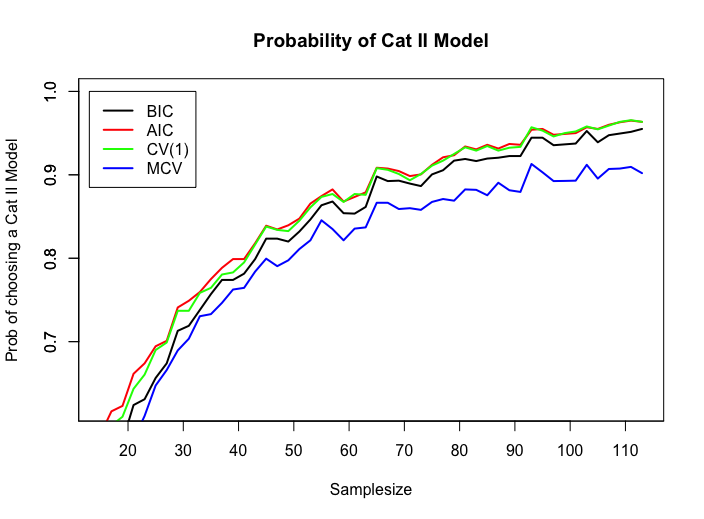
\includegraphics[width=1.3\textheight]{Simulation1.png}
\end{frame}
%The Graphic shows a graph for every Method
%We obtain that all Methods behave simalary, i.e The probabiltiy of selecting a Cat II model growth together with the samplesize and aproaching one very quickly.
%Moreover one can see that all methods behave similary for ceratin shocs in the datastructure
%%Christoph%%

%As we allready claimed out: For n large enought the Prob of choosing a Cat I model goes to Zero. Therfor we just can ignore all these models by choosing n large. 
%In the next simulation we concentrate on the probabilty of choosing a model of certain size within Cat II
%%Christoph%%
\begin{frame}
\frametitle{Thanks for your attention }
J. Scherer: s3jnsche$@$uni-bonn.de\\
V. Fritzsche: s6vifrit$@$uni-bonn.de\\
C. Zilligen: s3chzill$@$uni-bonn.de

\end{frame}


\end{document}